\title{Lab 6: Altium}
\author{Engineering 100-950}
\date{Winter 2020}
\documentclass[12pt]{article}
\usepackage[margin=1in]{geometry}
\usepackage{fancyhdr}
\chead{Written \& Edited by Arun Nagpal, Lyndon Shi, Scott Smith, Sarah Redman, Kitty Ascrizzi}
\usepackage{hyperref}
\usepackage{circuitikz}

\begin{document}
	\maketitle
	\thispagestyle{fancy}
	
    \section*{Calendar}
    \begin{table}[h]
        \begin{tabular}{lllll}
        Introduction to PCBs & 2/18/20  &  &  &  \\
        PCBs due for Peer Review         & 2:30pm on 2/25/20 &  &  &  \\
        Peer Reviews due after Lab     & 5pm on 2/26/20 &  &  &  \\
        Final PCBs Due    & 5pm on 2/27/20 &  &  &  \\
        PCBs Arrive for Assembly   & 3/9/20 &  &  &
        \end{tabular}
        \end{table}
    
	\section*{Introduction}
    In this lab, you will be designing your sensor board in its totality in \textbf{Altium Designer}, a PCB design software that is an industry standard. This design will be sent directly to manufacturers for fabrication, and you'll have your completed PCBs sent back to you to start constructing your payload after Spring Break! There is no postlab for this lab. Focus on making sure your design is good, and everything about your board works. Once the PCBs are ordered, you cannot make changes. Sometimes, we can work around mistakes manually. Sometimes, teams have needed to use an old PCB from previous classes. \textbf{Upon submission, if you fail any design rule checks, you will receive a 0 for this lab. This is true even if everything else is correct. You must pass all design rule checks to get credit for this lab.} 
    
    \section*{Participation}
    Working at a computer often can become a one person deal. It is important to avoid this during this lab. Our goal is for all students in this course learn the basics of Altium. When you are working on your PCBs, have at least one person spotting the person at the computer. This will help you share the work that goes into creating the PCB and eliminate mistakes that can render your finished product useless. We will be designating times in full class Altium sessions to rotate roles. Make sure all team members are involved and ready to rotate at any time! It is important that no team member works alone, even during office hours. This lab is two weeks long to allow you ample time to meet in groups of at least two and allow all members to spend some time on Altium.
    
    \section*{Preparing your Layout and Extra Sensor}
    The following are a few design specific notes you must keep in mind while laying out your Altium schematic:
    \begin{enumerate}
        \item All of our boards will use the same power architecture (See Figure 1). Keep the following in mind for power architecture:
        
        \subitem We will use a 5V and a 3V3 LDO. All items that need 5V power should get it from the output of the 5V LDO, not the Arduino. Same goes for the 3V3 LDO.
        
        \subitem Use the 5V pin on the Arduino to supply the Arduino with 5V from the output of the LDO. We use the 5V pin instead of the Vin pin because the Vin pin expects a voltage between 7-12 volts.
        
        \item To have enough analog pins available to incorporate your extra sensor, you will have to eliminate either your TMP36 or your Thermistor. Your team should consider which is more reliable and more suited to what you hope to measure. Then choose the best fit. 
        
        \item If your extra sensor uses I2C communication protocols, you must connect it to the analog pins pre-set for I2C communications. In the Arduino Nano, these are A4 (SDA pin) and A5 (SCL pin). See more on connecting I2C devices \href{https://www.lehelmatyus.com/691/sda-scl-arduino-nano-connecting-i2c-devices-arduino-nano}{(by clicking here)} Be sure you read through your extra sensor's documentation and/or hookup guide to understand whether it is I2C and if you will need the A4 and A5 I2C hookup pins.
    \end{enumerate}
    
    \begin{figure}[h]
    \begin{center}
    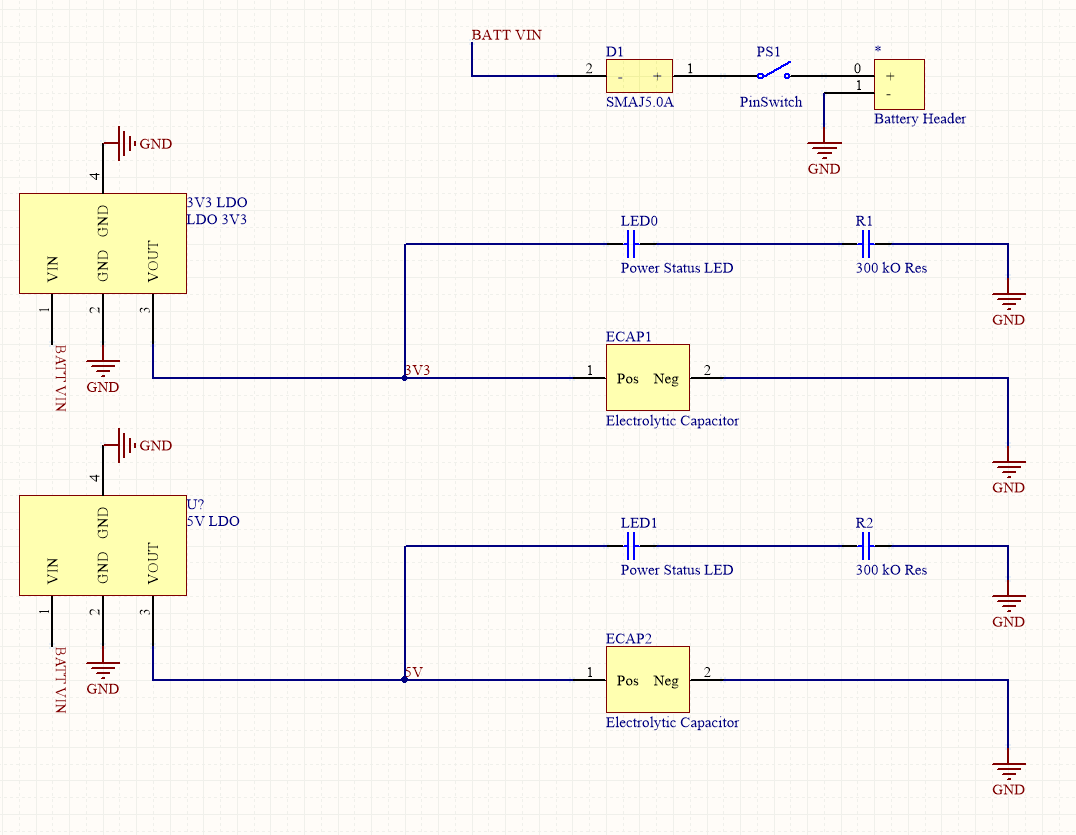
\includegraphics[scale = .3]{Figures/Altium_pwr.PNG}
    \caption{The power and voltage protection architecture of your board. The leftmost two components are LDOs, the top is 3.3V, and the bottom is 5V. D1 indicates a diode for battery protection.}
    \end{center}
    \end{figure}
    
    \section*{Altium}
    Altium as a software can be very complex, and as such, we have given you some tools to help simplify the process of constructing your PCB. The following pictures are taken from a free online tutorial provided by Altium: \href{http://www.altium.com/documentation/18.0/display/ADES/From+Idea+to+Manufacture+-+Driving+a+PCB+Design+through+Altium+Designer}{\underline{From Idea to Manufacture}}. You can learn more about this example there.\\
    
\noindent 
    Broadly, the workflow in Altium is divided up into three steps: Schematic, PCB, and Design Rule Check. The Schematic step is where you lay out the electrical schematic of your board. Using all the components, you define how they connect to each other, ground, and power. The PCB step is where you the physical layout of those components on the board. The electrical connections you set up in the schematic are shown for your reference, and you lay them down on your PCB physically as traces. That is, each trace you set corresponds to an electrical connection you outlined in your Schematic. The Design Rule Check step is when the software looks over your work and makes sure you aren't committing any errors or contradictions. This is inevitably the most frustrating part of using Altium, because you think you've done everything right, and the software is here to tell you that you haven't. It is important to note that design rule checks do not check whether you laid out your board the way you wanted, they will not notice if you accidentally connected your temperature sensor to your pressure sensor instead of the Arduino. You must double check this yourself. The design rule checks only check if your design is violating the physical and electrical laws associated with making a PCB.
    
    \subsection*{Schematic}
    You begin with an idea. A circuit or device that you'd like to realize in a PCB. The first thing you need to do is tell Altium the components you'll be using, and their relationships to one another. Consider the drawing of a `self-running a stable multivibrator' below.
    
    \begin{figure}[h]
    \begin{center}
    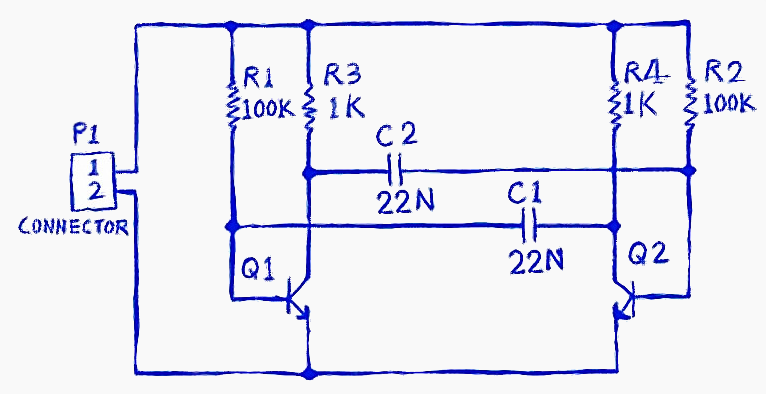
\includegraphics[scale=0.5]{Figures/Altium_astable.PNG}
    \caption{A drawing of a schematic, that pretty closely resembles the schematic you'd make in Altium.}
    \end{center}
    \end{figure}
    
\noindent 
Fig. 3 shows Fig. 2 as an Altium schematic. The schematic is defined in a document with the extension \textbf{.SchDoc}. 
\begin{figure}[h]
    \begin{center}
    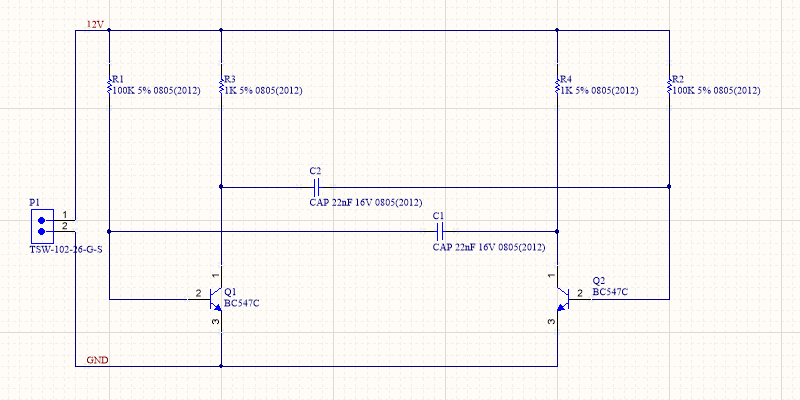
\includegraphics[scale=0.6]{Figures/Altium_sch_Wired.png}
    \caption{The schematic of an astable multivibrator as displayed through Altium.}
    \end{center}
    \end{figure}
Note that each component is defined with its own individual symbol. Capacitors, resistors, and transistors (Q1 and Q2), and some connectors (P1) are standardized and thus have pre-loaded symbols in the software, but for most of our components, that is not the case. We have additional libraries custom made by ENGR100 staff with our components pre-loaded, so, as we will discuss in the procedure, you can simply drag and drop them into place. 
    
	\subsection*{PCB}
    
    The PCB is designed as a separate document with the extension \textbf{.PcbDoc}. We can create a new PCB document and correlate it to our schematic. This will import all the components to the PCB document. Then, just as in the schematic document, we can manually place each footprint. As before, the footprints will be provided via a custom library we have prepared for you. \\
    
    
\noindent
Note the white lines that connect each of the footprints in Figure 4. These represent what pins on each part that should be connected via traces. This should be done manually, similar to the way that wires were drawn in the schematic. One notable difference is that physical traces should never be drawn at right angles - instead they should be at obtuse angles. This is to minimize field leakage and reflection at corners.\\

\noindent
Finally, we have a completed board! Altium creates a cartoon (Figure 5) that we can view before moving on to the final stage: Design Rule Check.

\begin{figure}[h]
    \begin{center}
    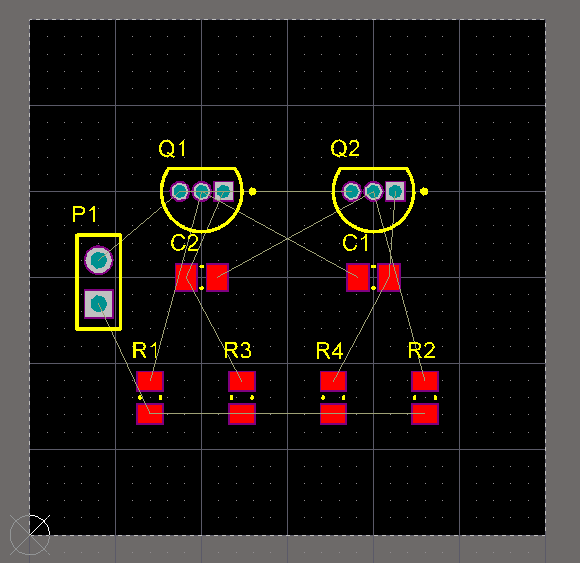
\includegraphics[scale=0.4]{Figures/Altium_pcb1.PNG}
    \caption{The PCB Layout in Altium.}
    \end{center}
    \end{figure}
    
    \begin{figure}[h]
    \begin{center}
    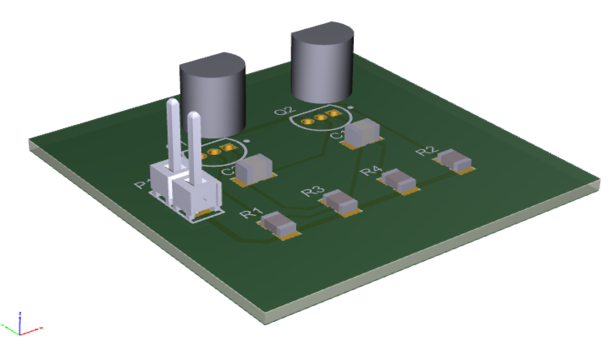
\includegraphics[scale=0.6]{Figures/Altium_pcb2.PNG}
    \caption{The completed multivibrator!}
    \end{center}
    \end{figure}

\subsection*{DRC}
    The DRC, or Design Rule Check is a way to check the validity of your PCB with respect to the Design Rules we create. More on this in the procedure.\\

    \begin{figure}[h]
    \begin{center}
    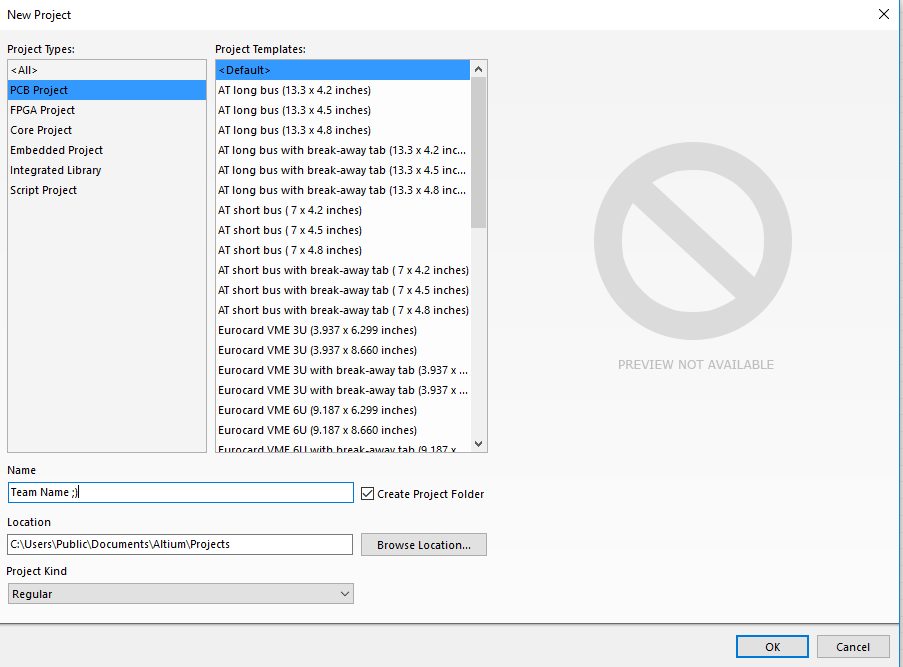
\includegraphics[scale=0.4]{Figures/Altium_newproj.PNG}
    \caption{The Project Creation Wizard popup. It should look something like this when you're done.}
    \end{center}
    \end{figure}
    
    \begin{figure}[h]
    \begin{center}
    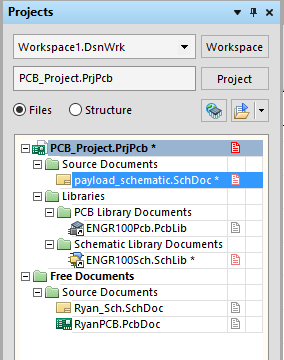
\includegraphics[scale=0.5]{Figures/Altium_projtab.PNG}
    \caption{The Project Tab should be on the left side of your screen}
    \end{center}
    \end{figure}
    
    \begin{figure}[h]
    \begin{center}
    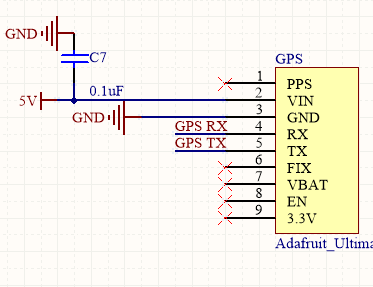
\includegraphics[scale=.7]{Figures/Altium_gpsnets.PNG}
    \caption{The GPS, connected using nets instead of wires}
    \end{center}
    \end{figure}
    
\section*{Procedure: Creating Your Design}
    \begin{enumerate}
    \item Open Altium Designer on a CAEN computer. Navigate to File $\rightarrow$ New $\rightarrow$ Project...
    \item Choose a regular PCB project using the default template. 
    \item Make sure the ``Create Project Folder" box is checked. This will designate a directory to save all of your project files in. The ``Location" field allows you to choose where this folder is created.
    \item Name your project something related to your team name or number, and click ``OK". See Fig. 6 for an example Project Creation.
    
    \item Now you should add two libraries we will give you. To do this, go to the Projects tab on the left side of the screen. A picture of this tab is shown in Fig. 7. If you see something else here, see if you can click the word ``Projects'' at the bottom left of the window.
    
    \item Right click your project name in bold and click Add Existing to Project. Navigate to your saved PCB libraries and select both of them.
    
    \item Look at the Projects Tab on the left side of the screen. Right click your project name in bold and click Add New to Project $\rightarrow$ Schematic. A blank piece of paper should appear on the screen. This is where you are to lay out your schematic drawing.
    
    A few instructions for laying out a schematic:
    \begin{itemize}
    \item  The 'Components: Final PCBs' spreadsheet on Canvas under Files / Labs / Lab 6 Altium Resources lists all components you might need for your system, their schematic names, and footprint names. It's important to note: all non-electrolytic capacitors, all 300 Ohm and 1 kOhm resistors and all LED's must use a C1206 capacitor footprint as indicated on this spreadsheet. 
    \item Go to Place $\rightarrow$ Part to place a component. Navigate to the library you would like to use with the dropdown menu. A keyboard shortcut is to simply press 'P' twice in a row.
    \item Rather than connecting everything with wires, use \textbf{nets} to connect your components. Nets are a convenient way to connect two pins without explicitly drawing a wire between them. Consider this example for the GPS (Fig. 8). You can place a net using Place $\rightarrow$ Net Label.
    
    This is a great way to make sure things don't get too messy.
    
    \item As you can see from the picture of the GPS, there's a capacitor in there that we haven't seen before. Since your board will be relying on raw battery power as its only means of operation, we are playing it safe and smoothing out any potential high frequency noise. So, for \textbf{all sensors}, tie a 0.1$\mu$F capacitor to the $V_{in}$ or $VCC$ line, which itself should output directly to ground.
    
    \item You must place one 3x1 header somewhere on your schematic, that connects to a 5V net, a 3.3V net, and GND. Call this header `Test Points.' It will be used to test your battery voltage.
    Headers can be found in the Miscellaneous Connectors Library.
    
    \item Your board requires significant power architecture. Lay out the the components shown in Fig. 1. The LEDs serve as status indicators and battery protection.

    \item To find the properties of a given component, double click its symbol on the schematic. A component-specific properties window will open up. Here you can adjust the part label, the value of the component (such as resistance or capacitance), and the \textbf{footprint} of the component. The footprint is a representation of how the component looks in real life - e.g. what actually will be on your board.You can add a footprint by clicking the corresponding Add button in the Component Properties window.
    
    \item Make sure to include the components and connections necessary to implement your extra sensor(s). Ask the IAs for help if you have questions on how these extra sensors should connect to your Arduino.
    \end{itemize}
    
    That's a lot to keep in mind! The path to success involves moving slowing and methodically through each component, writing out your schematic on paper beforehand, staying organized, and asking questions. If you're confused on what to do, please ask! \textbf{When you've finished your schematic, ask an IA to check it off and make sure it is correct.} Once they mark it off, you can move onto creating the PCB. It is in your best interest to have a clean and accurate schematic before moving forward. Even minor changes on the schematic can require substantial changes on your PCB to accommodate.
    \end{enumerate}
    
    \section*{Making the PCB}
    \textit{Pressing 1 on your keyboard takes you to the board design view. Pressing 2 takes you to the component layout screen. Pressing 3 takes you to the cartoon mockup screen. You should do your layout work (e.g. most of the work) in mode 2.}
    
    \begin{enumerate}
    \item To create a new PCB file, right click your project name under your Projects tab, click New $\rightarrow$ Add New to Project $\rightarrow$ PCB.
    \item Import your schematic components. Go to Design $\rightarrow$ Import Changes from Project name. Validate your changes, make sure you see only green check marks next to each change. Then execute them. By zooming in and out on your board (by pressing the mouse scroll button and moving around), you should see a big red box containing all of the components. You can drag and drop them onto the board, which is the black rectangle.
    
    \item Now we should adjust the size of our board. To do this, press 1 on your keyboard. Navigate to Design $\rightarrow$ Edit Board Shape. The board should be no bigger than 4.5-in to a side. You can toggle between Imperial and Metric units by pressing Q.
    
    \item We will add some design rules. Press 2 on your keyboard to ensure that you are on the component layout screen. Navigate to Design $\rightarrow$ Rules\dots
A PCB rules window should pop up. Set the following design rules:

    \begin{itemize}
    \item Electrical $\rightarrow$ Clearance = 6 mil 
    \item Routing $\rightarrow$ Width
        \begin{itemize}
            \item Minimum Width = 6 mil
            \item Preferred Width = 15 mil
            \item Maximum Width = 30 mil
        \end{itemize}
    \item Manufacturing $\rightarrow$ MinimumAnnularRing = 7 mil
    \item Manufacturing $\rightarrow$ HoleSize = 13 mil
    \end{itemize}
    
    \item Layout your components neatly on the board. Be sure to place your Arduino and OpenLog in such a way that you do not obstruct the port for the uploading cable or the SD Card opening. 
    \item To connect traces to your different components, navigate to Route $\rightarrow$ Interactive Routing. When you are placing a trace press 3 to toggle between your min, preferred, and max trace width as set in the design rules.  Recall from lecture that your board will contain two copper layers. These layers are referred to as the top and bottom layers, and are colored red and blue. Route all traces except the ground traces. We will route those later to our polygon pour ground plane, which we make last.
    
    \item When routing, all traces should default to 15mil if you implemented the Design Rules correctly. However, you should manually make a few of the power lines thicker, to compensate for the increased current flow through them. 
    
    \begin{itemize}
    \item Power lines to the Input of the LDO's = 30 mil.
    \item Output of the LDO's to the electrolytic capacitors and status LEDs = 25 mil.
    \end{itemize}
    \item Finally, we should pour a ground plane. Using the menu at the bottom of the PCB, select the bottom layer and cover it with a grounded polygon pour. You can now connect all your ground connections directly to this by using vias (no traces involved).
    
    \item Recall that you created a set of Design Rules before creating your PCB. The Design Rule Check (DRC) assesses your design in light of these rules, and highlights any discrepancies between your layout and those rules. Your DRC must return ZERO errors before your PCB can be considered complete.
    Design Rule Check can be run by navigating to Tools $\rightarrow$ Design Rule Check. Click Run Design Rule Check to run DRC. Generally, errors are highlighted in bright green.
    
    \item Once you have passed all design rule checks, take a screenshot of your error-free DRC screen
    
    \end{enumerate}
	
    \section*{Peer Review}
    \href{https://drive.google.com/drive/folders/1HiCb5Kfc1rcL4PkWGpplv0pV3mDflQRK?usp=sharing}
    In the second week of this lab, every student will be required to peer review the PCBs of three other teams. Each team must upload a single zip file containing all project files and a screenshot showing all DCRs passed to this designated Google Drive folder \href{https://drive.google.com/drive/folders/1HiCb5Kfc1rcL4PkWGpplv0pV3mDflQRK?usp=sharing}{(click here)} by 2:30pm on Tuesday, February 25th, 2020. Make sure that your PCB passes all design rule checks \textbf{before} submitting it to the Google Drive folder.
    
    In lab, each student will peer review three PCBs with rubrics provided on Canvas. Peer reviews are due by the end of your lab period.
    
    \section*{Final Deliverable}
    \href{https://drive.google.com/drive/folders/1HiCb5Kfc1rcL4PkWGpplv0pV3mDflQRK?usp=sharing}
    Your team will have 24 hours between 5pm on Wednesday, January 26th, 2020, and 5pm on Thursday, January 27th, to implement changes recommended by peer reviews. Then, rename your project with the ending '-FINAL' and re-upload the single zip file containing all project files and a screenshot showing all DRCs passed to this designated Google Drive folder \href{https://drive.google.com/drive/folders/1HiCb5Kfc1rcL4PkWGpplv0pV3mDflQRK?usp=sharing}{(click here)} by 5pm on Thursday, February 27th, 2020. \textbf{All design rule checks must be satisfied or you will receive a 0 on the assignment. This assignment MUST be finished on time or you will face significant difficulties completing the rest of the project.} Spend a lot of time ensuring that your design is correct. Do not hesitate to talk to the IAs or Professor Ridley.
    
\end{document}
